\documentclass[a4paper,11pt]{article}
\usepackage{a4wide}
\usepackage[ansinew]{inputenc}
\usepackage{pst-plot, pstricks,pstricks-add,pst-node, pst-tree}
\usepackage{graphicx}
\usepackage{bm}
\usepackage{natbib}
\usepackage{longtable}
\usepackage{rotating}
\usepackage{pdflscape}
%\usepackage{pdfdraftcopy}


%\usepackage{jurabib}
   %\jurabibsetup{  
     %authorformat=and  
    % commabeforerest,  
    % titleformat=colonsep,  
    % bibformat=tabular  
   %}  

\usepackage[bookmarks=true, bookmarksopen=true,
                bookmarksnumbered=true, colorlinks,citecolor = blue,
                filecolor=blue, linkcolor=blue, urlcolor=blue,
                plainpages=false,hyperindex=true,breaklinks=true]{hyperref}
\hypersetup{
        pdftitle={},
        pdfauthor={Anton Burger and Robert Ferstl},
        pdfsubject={},
        pdfkeywords={},
        pdfcreator={},
        pdfproducer={}
     }

%\usepackage{natbib}
%\usepackage{dingbat}
\usepackage{amssymb,amsmath,amstext}
%\usepackage{manfnt}

\setlength{\parindent}{0.0cm}                      % Absatzeinr�ckungen
\setlength{\parskip}{1.5ex plus 0.5ex minus 0.5ex} % Absatzabst�nde
%\renewcommand{\arraystretch}{1.5}                 % Zeilenabstand in Tabellen


\begin{document}
\title{Peak Load Pricing and Price Caps under Imperfect Competition - A Note\\\vspace{0.3cm}\emph{Draft version}\thanks{Please do not cite without consulting the authors.}}
\author{Anton Burger\thanks{\href{http://www.wu-wien.ac.at/regulierung}{Institute for Regulatory Economics, Vienna University of Economics and Business Administration,} \href{mailto:anton.burger@wu-wien.ac.at}{anton.burger@wu-wien.ac.at}}\hspace{1cm} Robert Ferstl\thanks{\href{http://www-finanzierung.uni-regensburg.de/}{Department of Finance, University of Regensburg,} \href{mailto:robert.ferstl@wiwi.uni-regensburg.de}{robert.ferstl@wiwi.uni-regensburg.de}}}
\maketitle
\abstract{Peak Load Pricing was combined with a two stage game under uncertainty. It was shown that imperfect competition leads to investment withholding relative to the welfare optimal benchmark. We use a discrete time Hamiltonian which allows us to interpret the shadow prices as expected scarcity rents which themselfes depend on the Cournot-Nash equilibria that clear the market. In a certain range, price caps were found to increase investments, as they mitigate the incentive to withhold investments to drive up prices whereby too low price caps led to sharp drops in investments due to the missing money problem.
\\
\\

\textbf{Keywords:} peak load pricing, investments, uncertainty, oligopoly, imperfect competition, price caps, electricity, dynamic games
\\
\textbf{JEL Codes:}
}

\section{Introduction}

In this note, we investigate how firms which act on a market where the conditions for peak load pricing are given would behave in the cases of a monopoly, a cournot oligopoly, perfect competition or price caps. With the ongoing deregulation of electricity markets, this question became pressing as it is still unclear how profit maximizing firms with market power would set capacities which used to be set by central planning before. However, our model setup is valid for all industries with limited storage possibilities or high storage costs and a high volatility of demand. This model is also suitable for industries in which expanding quantities beyond capacity is extremely expensive such as pipelines or other means of transport, the petrochemical industries or even hotels, restaurants or the market for real estate.
The basics of Peak Load Pricing are well established in theory and are summarized in \cite{Crew1986} but they are based on the assumption of central planning and so peak load pricing is only one building block used here.

Strategic interaction of firms must be accounted for as well. The seminal article when it comes to capacity choice prior to Bertrand competition is \cite{Kreps1983} who showed that firms would choose exactly the Cournot quantities in a deterministic two stage game in which firms first invest into capacities and then compete according to Bertrand. To combine peak load pricing and strategic interacion we have to use a framework in which firms play against nature (uncertainty) and against their rivals (strategic interaction). \cite{Gabszewicz1997} analyze investment under demand uncertainty with Cournot competition in the second stage and compare that to a Cournot game played in expected demand which they call the Cournot certainty equivalent game. They prove the existance of a symmetric subgame perfect equilibrium at which firms invest higher capacities compared to the Cournot certainty equivalent game.

Other recent literature on capacity investments is more focused on electricity markets. \cite{Genc2007}, \cite{Genc2007a} and \cite{Lise2008} discuss numerical models of electricity markets based on open loop games, but do not focus on economic explanations of the effects found. \cite{Murphy2005} offer a model related to the latter ones and compare formulations relying on different information structures (open or closed loop) with the perfect competition case.

Price Caps and their effect on investments were discussed in the literature already as they are a commonly proposed tool for the mitigation of market power on electricity markets about which there is a vast literature (see \cite{Ventosa2005} for an overview). It is a common preconception that Price Caps lower investments as they also cap possible scarcity rents firms might get if capacities are binding. This problem is called the missing money problem in the corresponding literature . Mainly in response to the missing money problem, various mechanisms to spur investments have been proposed. \cite{Cramton2006} give an overview on the missing money problem and proposed remedies.
\cite{Roques2006} investigate investment incentives under demand uncertainty and Price Caps in a real option framework. 

The contribution of this paper is the following: Our model uses a setup which is comparable to \cite{Gabszewicz1997} but we formulate the problem as a discrete time Hamiltonian. The first order conditions can be used to characterize the equilibrium and to see the effect different market structures or a Price Cap have on the behavior of the firms. The system of equalities and inequalities arising from the first order conditions of the firms is solved numerically as a mixed complementarity problem (MCP) to visualize some examples. The formulation we use also allows us to interpret the shadow prices directly as scarcity rents and avoids the tedious task of accounting in which demand states capacities are binding or not. We also compare Monopoly and Cournot Oligopoly solutions to a welfare optimal benchmark solution. Finally, we add another Player, the regulator, who can set a price cap to which firms react when they make their decisions.

\section{Peak Load Pricing in Oligopolies}

In our model, we make assumptions which are relaxed in some other work which deals with electricity markets. Contrary to \cite{Joskow2007} and \cite{Boom2007} we assume that efficient price rationing is always possible. It is also an implicit assumption that if capacity is binding, the price of electricity is equal to the willingness to pay of the marginal consumer\footnote{The consumers on the electricity wholesale market however, are not the end users but usually retailers and it might well be that they care less than their end users about electricity deliveries which had to be price rationed. A possible solution for this problem might be to make electricity retailers pay penalties for the value of lost load (VOLL). \cite{Burger2007} present a case study in which the direct regulation of supply security is investigated.}.

\subsection{The Model}

We use a linear demand function $\alpha^s- \beta Q^{s,t} $ and our assumption of constant marginal costs $c$ and capacity constraints evolves naturally from the Peak Load Pricing setup. $Q^{s,t}$ is the total quantity of $i\in N$ players on the market so we have $Q^{s,t}= \sum_{i\in I} q_{i}^{s,t}$. Quantity is allowed to differ over the different demand scenarios $s\in S$ which account for the uncertainty involved. We use $t\in 0,1$ to index the investment and market clearing phase between which Nature chooses it�s random variables (see figure \ref{fig:sequence} for an illustration).

\begin{figure}
	\centering
\psset{unit=1.0cm} 
  \begin{pspicture}(-1,0)(8,2)
  %\showgrid
  \tiny
  \textcolor{red}{
  \psline[linecolor=red]{>->}(0,1)(7,1)
  \multido{\rA=0.5+1.9,\iB=0+1}{4}{
  \rput(\rA,1.9){$\iB$}
  \psline[linecolor=red]{->}(\rA,1.8)(\rA,1.2)
  \psline[linecolor=red](\rA,1.1)(\rA,0.9)
  }
  \rput(7.5,1){Zeit}
  \uput{0.2}[-90](0.5,1){\parbox{1cm}{ Regulator sets Price Cap $\overline{p}$}}
  \uput{0.2}[-90](2.6,1){\parbox{1cm}{Firms Invest $t=0$}}
  \uput{0.2}[-90](4.4,1){\parbox{1cm}{Nature}}
  \uput{0.2}[-90](6.4,1){\parbox{1cm}{Market Equilibrium \\ $t=1$}}
 % \uput{0.2}[-90](6.5,1){\parbox{1cm}{Der Vertrag wird exekutiert}}
  }
  \end{pspicture}
  	\caption{Sequence of Events}
	\label{fig:sequence}
\end{figure}

Please note that we use different intercepts $\alpha^s$ to account for varying demand levels. Furthermore, we assume that $\alpha^l > c+ \Gamma$ such that quantities are always nonnegative. $\beta$ is the slope of the demand function. Each of the demand levels occurs with a certain probability $\rho_s$. The interpretation of $\rho_s$ is interesting as we could model a game where future demand is uncertain by postulating that $\sum_{s\in S} \rho_s =1$. Alternatively, we could set $\rho_s =1; \forall s$ thereby saying that there are different future demand states which will all occur with certainty. When we use $\rho_s$ in the first way, the term scenario is most appropriate for each $s \in S$. The term market state is better for the second way as this formulation can be used to approximate a load duration curve to solve a peak load pricing problem. In what follows, we will use market states and scenarios interchangeably. A combination of the two concepts is straightforward. 

The profit maximization problem of each firm $i$ looks as follows:

\begin{gather}
	\max \pi_i(q_{i}^{s,t},K_{i}^t,I_{i}^t)=
	\sum_{s\in S} \rho_s \left[ ((\alpha^s- \beta Q^{s,1}) - c) q_{i}^{s,1}  \right] - \Gamma I_{i}^{0} \label{eq:oligopmax2} \\
			\text{s.t.:} \  q_{i}^{s,1} - K_{i}^t \leq 0; \ \forall i,s \label{eq:capacitycon} \\ 
										  K^{1}_{i}  - K^{0}_{i}  - I_{i}^0 = 0 ; \ \forall i  \label{eq:state} \\
 										  q_{i}^{s,1}; K^t_{i}; I_{i}^0	\geq 0; \ \forall i,s,t  \nonumber
\end{gather}
For the sake of shortness and clarity, we do not solve for a market equilibrium at $t=0$ as this would not influence investments at $t=0$. When deciding on how much to invest, firms only consider the expected future market equilibrium and investments costs $\Gamma$. The possible Cournot quantities are limited by \eqref{eq:capacitycon}, the capacity constraint which has to hold for every player in every market state.

The two points in time in our model are linked by \eqref{eq:state}, which is the state equation. $K^{t}_{i}$, the state variable is the available capacity of player $i$ at time $t$ and $I_{i}^0$, the action variable, stands for investments. At this point, we would like to point out that introducing depreciation, scrap values and a discount rate would be conceptually straightforward but would only complicate notation without adding much insight.

The corresponding discrete time Hamiltonian looks as follows:

\begin{gather}
	 H_i(q_{i}^{s,t},K_{i}^t,I_{i}^t,\lambda_{i}^{s,1},u_{i}^1)= 
	 \sum_{s\in S} \rho_s \left[((\alpha^s- \beta Q^{s,1}) - c) q_{i}^{s,1} \right]	- \Gamma I_{i}^{0}  \\ \nonumber  
	  	- \lambda_{i}^{s,1}(q_{i}^{s,1} - K^{1}_{i}) \\ \nonumber
			- u_{i}^1(K^{1}_{i}  - K^{0}_{i}  - I_{i}^t)	\\  \nonumber
\end{gather}

We have used $\lambda_{i}^{s,1}$ for the shadow price of capacity of firm $i$ in demand state $s$ and $u_{i}^1$ as the slack variable for the state equation.

Our Hamiltonian leads to the following Karush Kuhn Tucker conditions:

\begin{gather}
 - \rho_s \left[ \alpha^s - \beta q_{i}^{s,1} - \beta Q^{s,1} - c \right] + \lambda_{i}^{s,1} \geq 0 \ \bot \ q_{i}^{s,1} \geq 0;\ \forall i,s \label{eq:foc1a}
\end{gather}

This conditions stems from $\frac{\partial H}{ \partial q_{i}^{s,1}}$. As $q_{i}^{s,1}$ is always bigger than zero (as we assumed that $\alpha^l > c+ \Gamma$), the first condition must be fulfilled with equality. So the first part of \eqref{eq:foc1a} can be rewritten as follows:

\begin{gather}
 \rho_s \left[ \alpha^s - \beta q_{i}^{s,1} - \beta Q^{s,1}\right]=  \rho_s c  + \lambda_{i}^{s,1} ;\ \forall i,s    \label{eq:foc1b}
\end{gather}

Which means that, for all market states and players, expected marginal revenue must be equal to marginal costs plus lambda, the scarcity rent in the short run market equilibrium. In the perfect competition benchmark case, marginal revenues would be $\alpha^s - \beta q^{s,1}$, so we see that quantities are distorted downwards in the case of an oligopoly and even more so in the case of a Monopoly where marginal revenues would be $\alpha^s - 2* \beta Q^{s,1}$.

$\tfrac{\partial H}{ \partial \lambda_{i}^{s,1}}$ tells us that lambda is greater than zero if capacities are binding and grows larger, the more capacities are constrained.

\begin{gather}
 - q_{i}^{s,1} + K^t_{i} \geq 0 \ \bot \ \lambda_{i}^{s,1} \geq 0 ; \forall \ i,s \label{eq:foc2}
\end{gather}

$\tfrac{\partial H}{ \partial K^1_{i}}$, and $\tfrac{\partial H}{ \partial I_{i}^{0}}$ look as follows.

\begin{gather}
  -\sum_{s\in S}  \lambda_{i}^{s} + u_{i}^1 \geq 0 \ \bot \ K^1_{i} \geq 0 ; \forall i,k \label{eq:foc3} \\
 \Gamma - u_{i}^1 \geq 0 \ \bot \ I_{i}^{0} \geq 0 ;\forall i \label{eq:foc4}
\end{gather}

As $K^1_{i}$ is bigger than zero in any sensible case (as quantities are always bigger than zero, capacities are so too), the first part of \eqref{eq:foc3} will hold with equality. So $u_{i}^1$ indicates how much additional revenue a firm generates if capacities are increased by one unit as it is the sum of the shadow prices in the respective demand states. \eqref{eq:foc4} makes sure that investments are made until the marginal revenue from investments is equal to investment cost and that no investments are made if $\Gamma$ is bigger than $u_{i}^1$. Here, the real option character of the problem can be seen. Investments are only made, if the future expected gains outweigh the future costs. Finally, $ \tfrac{\partial H}{ \partial u_{i}^1} $ gives back the state eqation.

\begin{gather}
K^1_{i} -  K^0_{i} - I_{i}^{0}  = 0 \ \bot \ u_{i}^1 \ \mbox{\textit{free}}; \label{eq:foc5}  \forall i
\end{gather}

To have a look at the overall picture, consider \eqref{eq:foc1b}, \eqref{eq:foc3} and \eqref{eq:foc4} once again. Quantities and thereby investments are increased, until expected scarcity rents are equal to investment cost:

\begin{gather}
\sum_{s\in S}\lambda_{i}^{s} = \Gamma \label{eq:invcondition};  \forall i
\end{gather}

What we call scarcity rents is the difference between marginal costs and marginal revenues in any market form so our definition of scarcity rents is wider than the definition of scarcity rents in classical Peak Load Pricing. The reason why investments are lower under imperfect competition is that marginal revenues, and thereby scarcity rents decrease quicker in quantities in the case of imperfect competition. At the solution, there could be scarcity rents from one, two or $S$ market states depending on how demand is distributed. As under imperfect competition prices are above marginal revenues, high prices (above marginal costs) are not necessarily an investment incentive. The investment incentive only stems from the difference between marginal revenues and $c$. This result also means that, apart from investment withholding, firms also engage in withholding existing capacities to increase prices in low demand periods.

\subsection{Numerical Solutions}

To solve our model, we use the fact that the system of equalities and inequalities from the Karush Kuhn Tucker conditions can be conceived as a Mixed Complementarity Problem (MCP). These types of optimization problems can be implemented in GAMS (General Algebraic Modeling System) and solved with the PATH solver (see \cite{Ferris2000}).

\subsubsection{Peak Load Pricing}

The numerical values we use for our examples are given in table \ref{tab:note}. The first example in figure \ref{fig:1} considers a peak load pricing problem as $\rho_s = 1$ in both cases. $D^h$ and $D^l$ are the demand curves for the peak and off peak period respectively. $MR^M$ depict marginal revenues for the monopoly case and the black (lowest) horizontal line are short run marginal costs ($c$). The dashed vertical lines are the capacities of choice in the perfect competition ($K^1_{PC}$), the four player oligopoly ($K^1_{Olig}$), and the monopoly ($K^1_{Monop}$) case, whereby capacities are highest in the optimum and lowest in the monopoly solution.

The perfect competition solution is already known from peak load pricing. Capacities are expanded until marginal revenues from an additional unit of capacity, which is equal to the price, is equal to long run incremental costs ($c+\Gamma$). The long run incremental costs are illustrated by the highest horizontal red line. As it should be under peak load pricing, the off peak price ($p_{l,1}^{c}$) is equal to $c$. Note that \eqref{eq:invcondition} holds as scarcity rents (the difference between $p^c_{h,1}$ and $c$) are equal to $\Gamma$. 
%It is easy to verify that \eqref{eq:optpc} holds as well.

At the monopoly solution, prices ($p^c_{o,1}$) are 100.3 in peak, and 55.3 in off peak periods. Although the costs of additional units of capacity could be covered easily, a monopolist would exactly invest the amount shown as the difference between marginal revenues of the monopolist and it�s marginal costs is exactly equal to $\Gamma$ and so \eqref{eq:invcondition} holds again.

As expected, the 4 player Cournot-Nash equilibrium lies inbetween. At this point, \eqref{eq:invcondition} holds for all the four players in our example although this cannot be seen directly as we cannot draw the respective marginal revenue curve. The peak price of 70.5 can be seen directly, as capacities are binding in peak periods whereby the off peak price of 28.5 can not be read from figure \ref{fig:1} as the marginal revenues of an oligopolist cannot be drawn here. As this price is higher than $c$ it tells us that firms engage in withholding existing capacities in off peak periods.

Figure \ref{fig:2} considers a case where peak and off peak periods diverge less in an otherwise unchanged setup. Now, at all three solutions, capacities are binding in both market states. Again, \eqref{eq:invcondition} holds at the perfect competition solution. $p^c_{h,1}$ is much lower now, as some part of the fixed costs are now covered by $p^c_{l,1}$ as well, although peak periods still have to cover a higher share of the fixed costs. Specifically, $p^c_{h,1}$ is now lower than long run incremental costs $c+\Gamma$. The rest of the interpretation of figure \ref{fig:2} are along the lines of figure \ref{fig:1}.

\subsubsection{Competition under Uncertainty}

In the next example, we set $\rho_h = \rho_l = 0.5$ to model a two stage game under uncertainty. \ref{fig:3} can be interpreted along the same lines than the other two figures but now, we have to think in terms of expected marginal revenues which have to be equal to marginal costs. We also solved the same game by using an expected demand function and came to the same conclusion as \cite{Gabszewicz1997} as our stochastic solution yielded higher equilibrium investments than the certainty equivalent game.

\section{Adding Price Caps}

We now add another player, the regulator, who can announce a price cap before the first stage decision of the firms. 

\subsection{Modeling Price Caps}
This changes the optimization problem of the players and adds an additional constraint.

\begin{gather}
	\max \pi_i(q_{i}^{s,t},K_{i}^t,I_{i}^t, \overline{p})= \label{eq:pcmax1}
	\sum_{s\in S} \rho_s \left[ ( \min{(p_{s,1}^{o},\overline{p})} - c) q_{i}^{s,1}  \right] - \Gamma I_{i}^{0}  \\
			\text{s.t.:} \  p_{s,1}^{o} - \overline{p} \leq 0; \forall s,t \label{eq:pcconstraint}
\end{gather}

We now defined the price under imperfect competition at time $t$ and scenario $s$ as $p_{s,1}^{o}= \alpha^s - \beta Q^{s,1}$ and the price cap as $\overline{p}$. \eqref{eq:capacitycon}, \eqref{eq:state} and the nonnegativity constraints remain the same. From now on, we assume that there are two demand states $s \in h,l$ with $\alpha^h > \alpha^l$. This problem cannot be solved directly by the method we propose as the $\min$ operator leads to a nondifferentiable objective function. The $\min$ operator means that a firm either gets the market equilibrium price, which depends on quantities, or the capped price, which is independent of quantities as long as the price cap is binding. So we propose a two stage algorithm to solve the model for different levels of the price cap.

\subsubsection{Stage one}

First, consider the maximization problem without the price cap constraint. Consider the price under perfect ($p_{s,1}^{c}$) and imperfect competition.

\subsubsection{Stage two: Continue with one of the three cases}

\paragraph{Case 1 }If $p_{h,1}^{o} \leq \overline{p}$ the price cap is not binding and we can stop here. 

\paragraph{Case 2}If $ p_{h,1}^{c} \geq  \Gamma + c$ and the price cap is binding.

Case 2 is given if the optimal peak price $p_{h,1}^{c}$ is bigger than long run incremental costs $\Gamma + c$. As we will see later, under certain parameter constellations this might not be the case.

\subparagraph{Case 2a} If $\overline{p} \geq p_{h,1}^{c}$

in this case, the objective function is

\begin{gather}
	\max \pi_i(q_{i}^{s,t},K_{i}^t,I_{i}^t, \overline{p})= \label{eq:pcmax2}
	\sum_{s\in S} \rho_s \left[ (p_{s,1}^{o} - c) q_{i}^{s,1}  \right] - \Gamma I_{i}^{0}  \\  \nonumber 
\end{gather}

with \eqref{eq:pcconstraint}, \eqref{eq:capacitycon} and \eqref{eq:state} as constraints. In this interval, there is no discontinuity in investment behavior and we can solve the model. Below $p_{h,1}^{c}$, the peak period price under perfect competition, firms cannot cover their fixed costs in peak periods any more, investments will jump back and we will have to use a different model formulation. 

Under \eqref{eq:pcmax2}, \eqref{eq:foc1b} changes to:

\begin{gather}
 \rho_s \left[ \alpha^s - \beta q_{i}^{s,1} - \beta Q^{s,1}\right] + \beta \psi_s =  \rho_s c  + \lambda_{i}^{s,1}   ;\ \forall i,s  \label{eq:foc1c}
\end{gather}

Whereby $\psi_s$ is the slack variable for the price cap constraint which is bigger than zero if and only if the price cap is binding. The lower is the price cap, the higher is $\psi_s$ and the more quantities are "`distorted"' upwards. The other first order conditions (\eqref{eq:foc2} to \eqref{eq:foc5}) remain unchanged. As quantities are distorted upwards, investments are distorted upwards too. We can see from \eqref{eq:foc1c}, that the price cap could be set such that the right hand side is equal to the perfect competition result. The economic interpretation of this is that a price cap takes away the incentive to raise prices by reducing quantities and so it also reduces the incentive to raise prices be reducing investments. Under perfect competition, firms are willing to invest as long as there is a small positive return an an additional unit invested. For our case this means that firms will increase investments until the maximum market demand at the price cap is reached $Q^{h,1}=\tfrac{\alpha^s-\overline{p}}{\beta}$ whereby $Q^{h,1}$ could be the Output of a monopolist or several oligopolists.

The effect of a price cap can also be seen from the viewpoint of strategic variables the firm possesses. If there is no price cap, price - quantity combinations can be chosen subject to market demand and the behavior of competitors. Under a binding price cap however, only quantity remains a strategic variable.

Consider figure \ref{fig:1}. The red diamonds along $D^h$ above $c+\Gamma$ are the solutions of \eqref{eq:pcmax2} under the respective price caps. If the price cap is set marginally above $p_{h,1}^{c}$, the firms earn a small positive amount on every unit they invest until they reach the demand curve. Investing this additional units does increase the profit of firms, as in the low demand period, they can still withhold capacities to optimize profits there. In figure \ref{fig:1}, we see a situation in which a monopolist would be constrained by the optimal price cap in low demand periods as well, whereby the oligopoly price in the low demand period would be 28.5. Notice that at this point, firms still earn nonnegative profits as prices in the low demand period are above marginal costs. So even if the optimal capacity can be reached by a price cap, the first best solution can not. 

The red diamonds along the high demand curve in \ref{fig:3} can be interpreted in a similar way. Here, at a price cap slightly above $p_{h,1}^{c}$, expected gains in peak and off peak periods are slightly above investment cost and so firms invest until the optimal capacity is reached. In this example, neither the oligopoly, nor the monopoly price is constrained by $\overline{p}$ in the off peak period.

We now want to investigate the optimal price caps a bit further. Under perfect competition (welfare optimum), \eqref{eq:invcondition} can be written as $\rho_l (p_{l,1}^{c}-c)+ \rho_h(p_{h,1}^{c}-c) = \Gamma $ as prices are equal to marginal revenues. If the price cap is only binding in the high demand period, we can replace $p_{h,1}^{c}$ by $\overline{p}$, and solve for the optimal price cap.

\begin{gather}
p_{h,1}^{c} = \overline{p}^{opt} =  \frac{\Gamma - \rho_l(p_{l,1}^{c}-c) }{ \rho_h } + c \label{eq:optpc1}
\end{gather}

\eqref{eq:optpc1} can be interpreted as follows: At $\overline{p}^{opt}$ the firm must be allowed to cover marginal costs, plus investment costs which are not covered by expected scarcity rents that arise from the other period. It is easy to verify that \eqref{eq:optpc1} describes the optimal price cap in the third example and thereby also provides an intuition for that.
Please notice that this formulation is only valid if the price cap does not become binding in the off peak period also. If the price cap becomes binding in the off peak period as well, we have to replace $p_{l,1}^{c}$ by $\overline{p}$ as well and we get

\begin{gather}
p_{h,1}^{c}= \overline{p}^{opt} =  \tfrac{\Gamma}{(\rho_h+\rho_l)}+c \label{eq:optpc2}
\end{gather} 

This means that we have the same price in both periods and marginal costs plus a share of capacity costs has to be covered by the price cap.

Summarizing we can say that under case 2, prices at $p_{h,1}^{c}$ which can be understood by \eqref{eq:optpc1} and \eqref{eq:optpc2} lead to optimal investments, but nut to a first best solution. However, the financial viability of the firm is not undermined if price caps are lowered further as there are still profits from low demand periods. The next part explores this case.

\subparagraph{Case 2b }If$c+\tfrac{\Gamma}{(\rho_h+\rho_l)} \leq  \overline{p} \leq p_{s,1}^{c}$

If $\overline{p}$ is lower than \eqref{eq:optpc1}, firms cannot cover investment costs in peak periods and although they could cover the costs by cross subsidization from low demand profits, they have no reason to do so. As already mentioned, the literature calls this the missing money problem (see \cite{Cramton2006}). So firms would reduce investments until \eqref{eq:invcondition} holds again. This means that there is a jump in the relationship between investments and price caps. Now, for every unit firms sell in peak demand periods, they get $\overline{p}-c$ which does not cover investment costs. So we can see it as a subsidy the firm takes into account when deciding on how to choose investments with respect to the low demand period. So the objective function becomes:

\begin{gather}
	\max \pi_i(q_{i}^{s,t},K_{i}^t,I_{i}^t, \overline{p})= \label{eq:pcmax3}
	 \rho_h \left[ (\overline{p}-c) q_{i}^{l,1}  \right]+ \rho_h \left[ (p_{l,1}^{o} - c) q_{i}^{l,1}  \right] - \Gamma I_{i}^{0}  \\  \nonumber
\end{gather}

The constraints remain \eqref{eq:pcconstraint}, \eqref{eq:capacitycon} and \eqref{eq:state}. Finally, if $\overline{p}$ is below $c+\tfrac{\Gamma}{(\rho_h+\rho_l)}$, no investments are carried out any more.
The behavior of firms under a lower than optimal price cap is interesting. Consider figure \ref{fig:1}. If the price cap is lower than long run incremental costs, firms are not willing to invest the optimal capacity any more as they would incur a loss on every additional unit they invest in. The lower red diamonds describe the behavior of a monopolist under a too low price cap. If $\overline{p}$ is slightly below $p_{h,1}^{c}$, $\overline{p}$ is binding in both periods so the monopolist is not willing to supply more than the market demand at $\overline{p}$. So capacity investments will be exactly equal to the market demand at $\overline{p}$. If $\overline{p}$ is lowered further, investments would increase again (the incentive to withhold investments is destroyed by the price cap) until $c+\tfrac{\Gamma}{(\rho_h+\rho_l)}$ is reached but optimal capacities cannot be reached any more.
The blue points describe the behavior of a four player oligopoly. Under a price cap slightly below $p_{h,1}^{c}$, investments are higher than in the monopoly case, as off peak marginal revenues of oligopolists plus the "`subsidy"' from the high demand period are enough to sustain a higher investment level. As this "`subsidy"' is lowered, investments are so too. At one point, $\overline{p}$ is low enough to be binding in both periods and the oligopoly and monopoly investment decisions are the same again.
\ref{fig:3} can be read similarly but with expected marginal revenues and expected "`subsidies"'. Notice that in the monopoly case (the lower red diamonds), after the jump in investments the latter go back until marginal revenues of the monopolist are high enough such that \eqref{eq:invcondition} holds again. Additionally, we drew the behavior of a 2 and 4 player oligopoly.

Summarizing, we can say that under case 2, $\overline{p} \leq p_{s,1}^{c}$ is never optimal.

\paragraph{Case 3}If $ p_{h,1}^{c} \leq  \Gamma + c$ and the price cap is binding. 

There are parameter constellations, where long run incremental costs are bigger than $p_{h,1}^{c}$. If this is the case, an optimal price cap has to be below long run incremental cost too. At such a price cap however, it is not possible to cover $\Gamma + c$ by $\overline{p}$ by definition and so firms cannot be induced to invest until capacities are equal to $ D^h( \overline{p})$. Instead, firms will stop investing when they reach $D^l( \overline{p})$. So we can see the revenue the firms get for peak demand sales as a mere subsidy which again leads to formulation \eqref{eq:pcmax3}. It can be seen in figure \ref{fig:2} what happens if $\overline{p}$ is lowered from the point where the discontinuity occurs, $\Gamma + c$, downwards. Again, the behavior of a monopolist differs from the 4 player oligopoly until the price cap is binding in both periods in the oligopoly too. Contrary to case 2, optimal investments cannot be reached now. Another difference is that in case 3, the optimal price cap is not at $p_{h,1}^{c}$, but at the minimum possible $\overline{p}$ at which firms are still willing to invest $c+\tfrac{\Gamma}{(\rho_h+\rho_l)}$.

All possibilities are summarized in the following table. Under Case 2 optimal capacities are possible, whereby under case 3 only a second best price cap, which is lower than the optimal peak price under perfect competition can be set.

\begin{table}[htbp]
	\centering
\begin{tabular}{ccc}
        &  Case 2  & Case 3  \\
        & $c+\Gamma \leq p_{h,1}^{c}$ & $c+\Gamma > p_{h,1}^{c}$ \\
\hline
\multicolumn{ 1}{c}{$\overline{p} \geq p_{h,1}^{c}$} & optimal capacities possible  & \multicolumn{ 1}{c}{not optimal} \\

\multicolumn{ 1}{c}{} & at $\overline{p} = p_{h,1}^{c}$ & \multicolumn{ 1}{c}{} \\
\hline
\multicolumn{ 1}{c}{$\overline{p} < p_{h,1}^{c}$} & \multicolumn{ 1}{c}{not optimal} & second best price cap \\

\multicolumn{ 1}{c}{} & \multicolumn{ 1}{c}{} & at $c+\tfrac{\Gamma}{(\rho_h+\rho_l)}$ \\
\hline
\end{tabular}  
\end{table}

%Information Structure - Open Loop and Stochasiticity - zwischen Open und Closed Loop ist in dieser Formulierung eh kein Unterschied oder? Weil die Ausgangswerte K0 ja gegeben sind und ich nur einen Schritt davon weitergehe.
%Assuming an interior solution, the FOC look like: H strich = 0 
%Scrap Values are normalized to zero - fixed costs are the fixed costs for a year
%There Could be a market clearing at T=0 as well but as this has no effect on investments, we leave it away
%Verify whether the Hamiltonian is concave wenn konkav, dann Optimum
%Show that the Hamiltonian is not concave any more


\section{Conclusion}

In this paper, we combined Peak Load Pricing with a two stage oligopoly game under uncertainty. It was shown that as players consider their marginal revenues when deciding to invest, imperfect competition always leads to investment withholding relative to the welfare optimal benchmark. The game we solved can be interpreted as Peak Load Pricing under imperfect competition, or as imperfect competition under uncertainty, depending on how weights are chosen. The method we use makes it possible to interpret the shadow prices as expected scarcity rents. Whereby expected scarcity rents depend on the Cournot-Nash equilibria that clear the market.
Another advantage of our methodology is that is allows us to introduce a price cap which changes the market equilibrium and thereby also investments which are made on the bases of expected market equilibria. Price caps that are not too aggressive were found to increase investments, as they mitigate the incentive to withhold investments to drive up prices. Too low price caps however, led to the missing money problem and induced sharp reductions in investments. In some parameter constellations, it is possible to set a price cap such that capacities are set at the welfare optimal level. In other parameter constellations only a second best price cap can be set. In the one case or the other, a regulator would have to have a lot of information to set a well working price cap.

$\overline{p}=5$\\

$\overline{p}=3$ \\

$p^h_{Monop}$ \\

$p^l_{Monop}$ \\

$p^h_{Olig}$\\

$p^l_{Olig}$\\

$p^h_{PC}$\\

$p^l_{PC}$\\

$$

$q_1$ \\

$q_2$ \\

$R^h_1$ \\

$R^l_2$ \\

$R^l_1$ \\

$R^h2$ \\

$K_1$ \\

$K_2$ \\

$K_1$ \\

$K_2$ \\

$K_2^{PC}$ \\

$K_1^{PC}$ \\

$R^{h,PC}_1$ \\

$R^{h,PC}_2$ \\

$PC^{h}$ \\

$PC^{l}$ \\

$\frac{\lambda}{\beta}$

m�gliche Nash Equilibria
%------------------------------------------------------

\markboth{References}{References} %\frenchspacing
\bibliographystyle{chicago}
%\nocite{*}
\bibliography{../electricity}

\appendix
\newpage

\section*{Appendix}


\begin{table}[h]
\begin{center}

\begin{tabular}{lccc}
\hline      
  & Example 1    & Example 2     & Example 3  \\
\hline  
     $\Gamma$ &             40 & 40 & 40 \\

         $c$ &             10.6 & 10.6 & 10.6  \\

      $\beta$ &             0.0077 & 0.0077 & 0.0077  \\

     $\alpha^h$ &          150 & 150 &  150 \\

      $\alpha^l$     &        100 &        140 &        100 \\

      $\rho_s$ &        1 &1&       0.5 \\
      \hline 
\end{tabular}  
\end{center}
	\caption{Parameters for the examples}
		\label{tab:note}
\end{table}

\begin{figure}[h]	
	\centering
		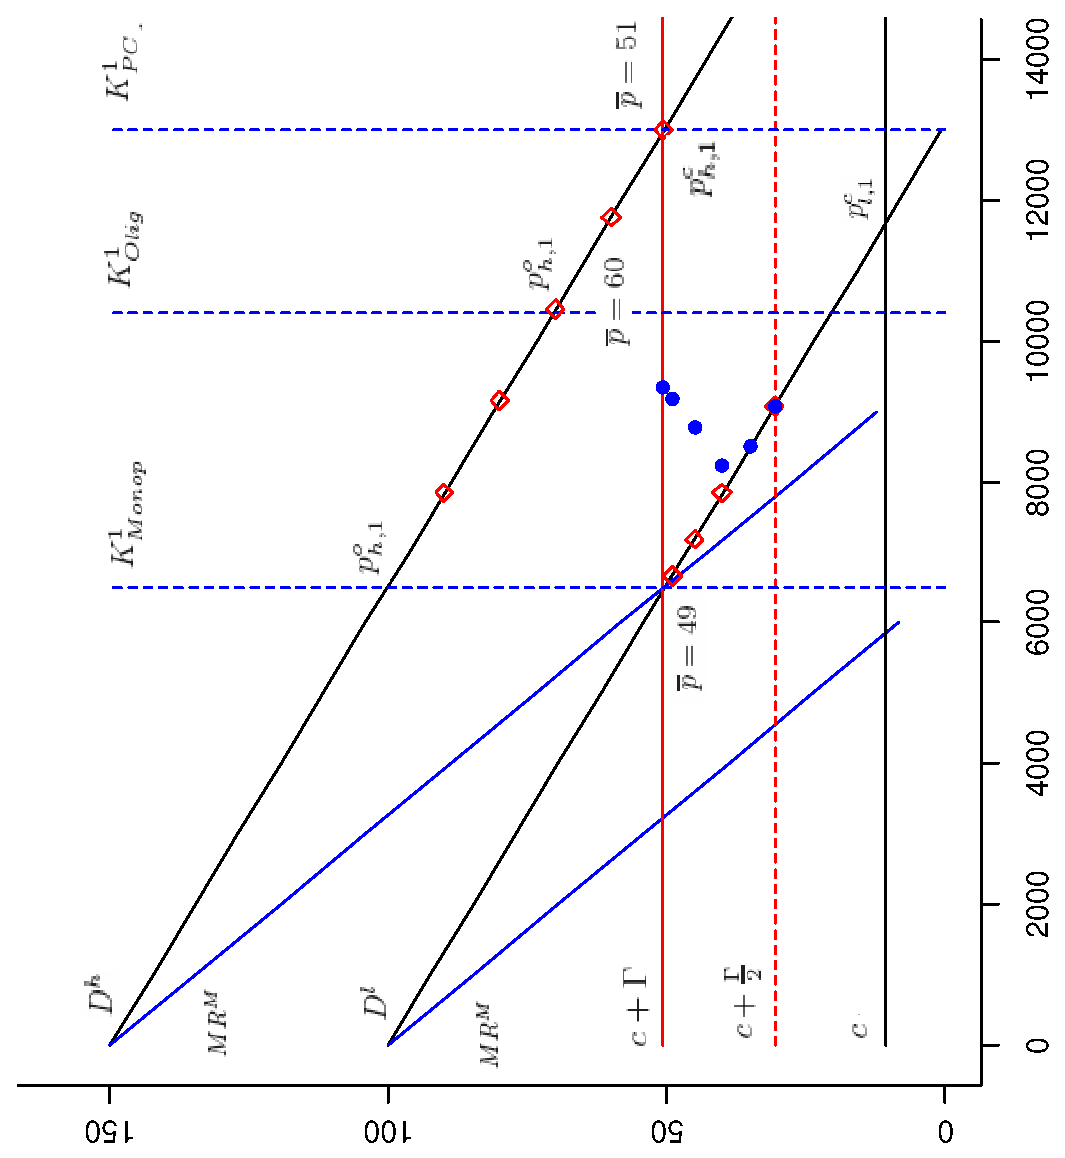
\includegraphics[width=0.6\textwidth, angle=270]{44}
	\caption{Numerical example 1}
	\label{fig:1}
	\scriptsize Source: own calculations
\end{figure}

\begin{figure}
	\centering
		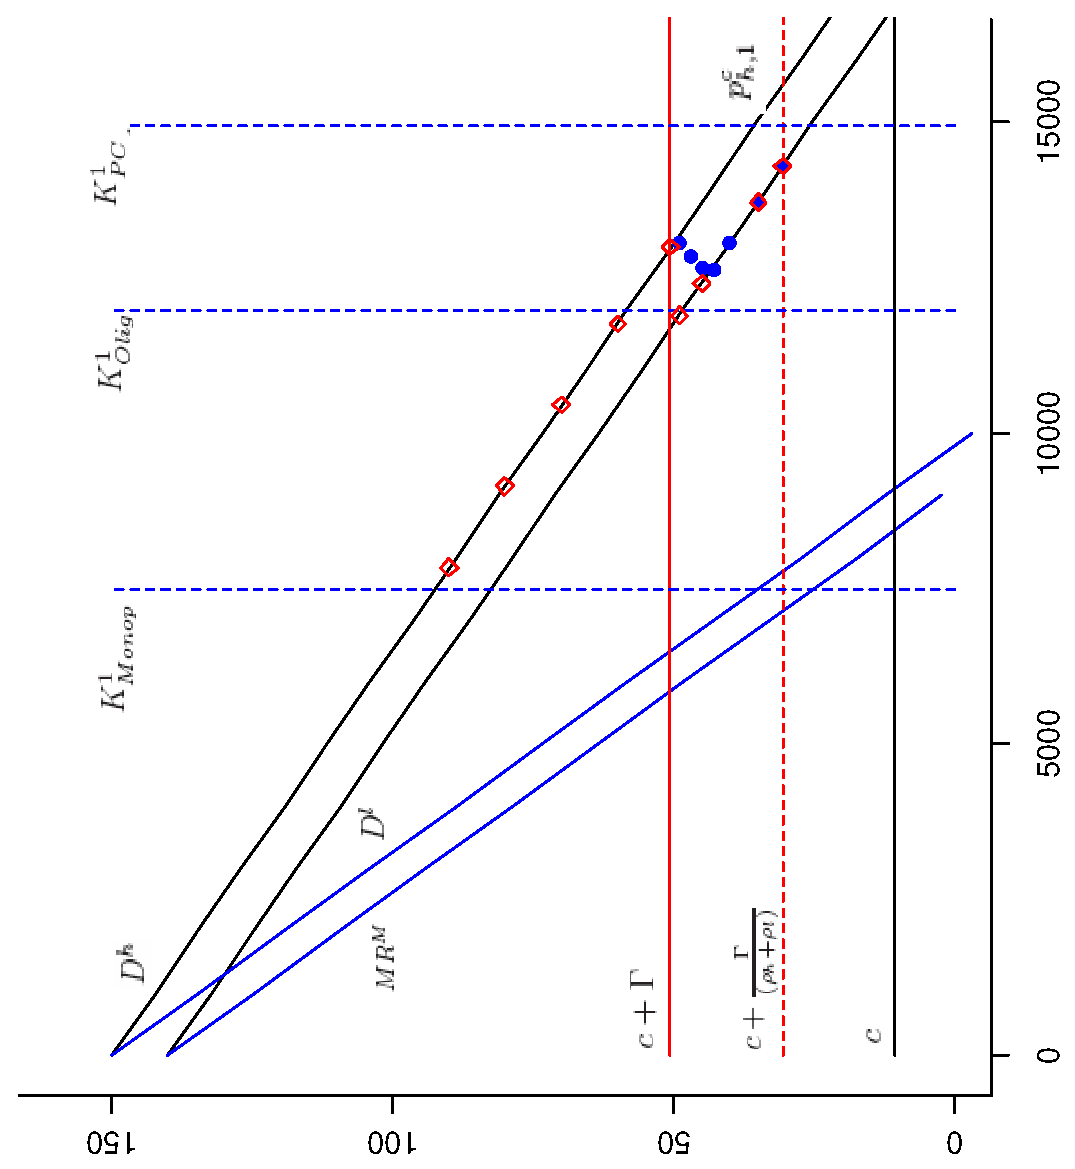
\includegraphics[width=0.6\textwidth, angle=270]{66}
	\caption{Numerical example 2}
	\label{fig:2}
	\scriptsize Source: own calculations
\end{figure}

\begin{figure}
	\centering
		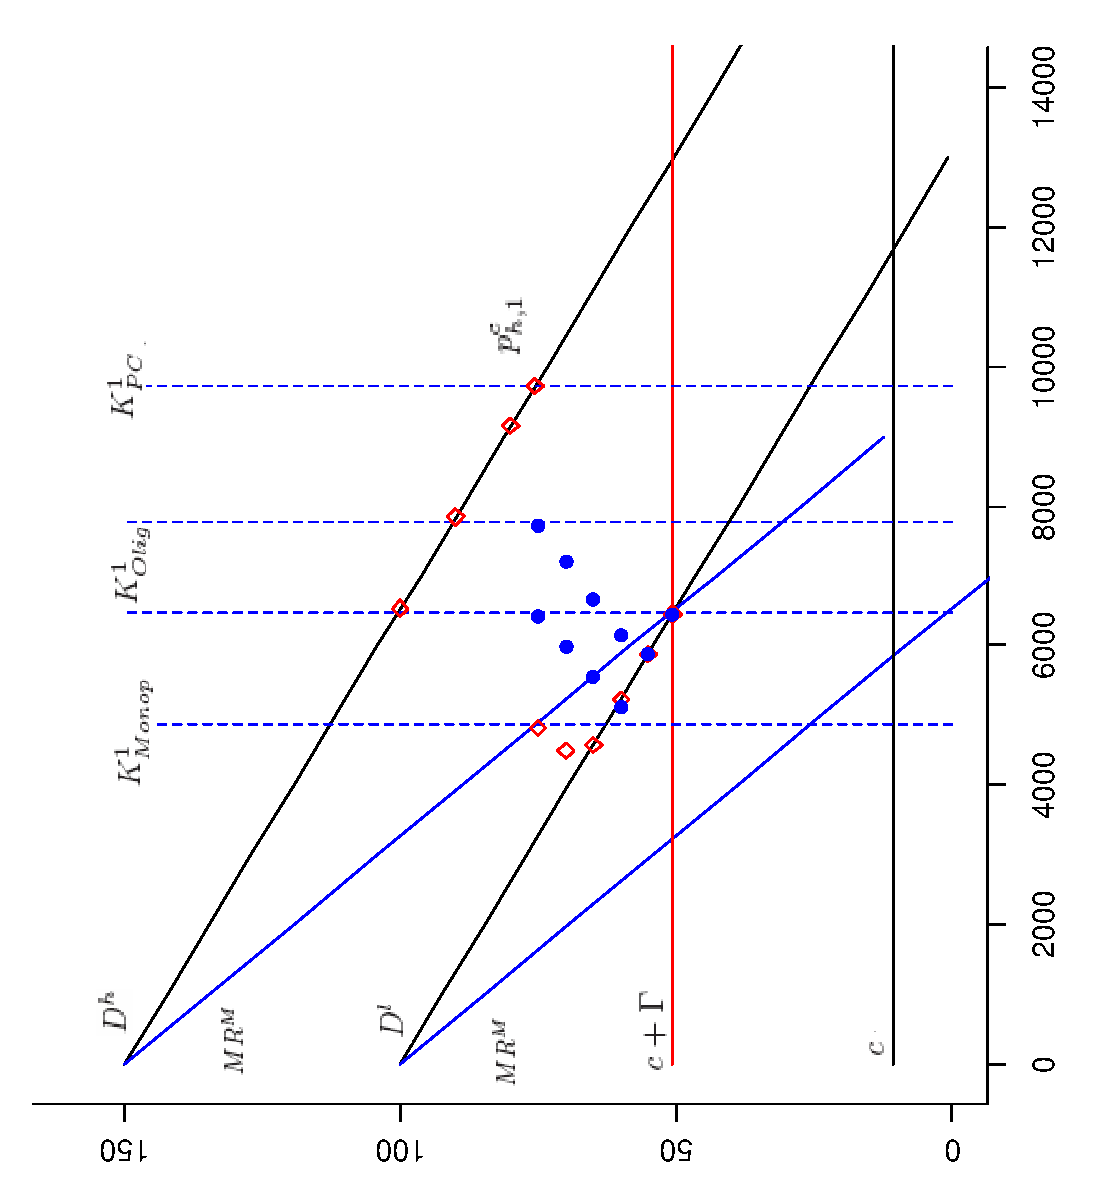
\includegraphics[width=0.6\textwidth, angle=270]{55}
	\caption{Numerical example 3}
	\label{fig:3}
	\scriptsize Source: own calculations
\end{figure}

\end{document}

%%% Local Variables: 
%%% mode: latex
%%% TeX-master: t
%%% End: 
